\section{Metal-covered handsets}
\label{sec:metal_cover}
Previous section explains the physical principles of an antenna. This section focuses on the recent antenna research, and more specifically, in designed antennas for metal-covered mobile phones. Metal-covered handheld devices are already popular, but mobile phones having metallic structure are still becoming more popular. In this section, the possible antenna types and design techniques as well as different styles of metal coverings are explained by introducing examples presented in recently published scientific articles.

\subsection{Antenna techniques in metal-covered handsets}
\label{sec:metal_rim}
Using metal rim on the sides of a handset improves robustness and strength of the device, and also makes the appearance of the phone modern \cite{ban_dual_loop, hsu_compact, yuan_slot}. However, it affects the performance of antennas significantly. As the rim is made of metal, i.e.\ conductive material, it couples with the internal antennas and harms their radiation performance \cite{ban_dual_loop}. Presence of metal near the antenna weakens the impedance matching by adding large capacitance to antenna's input impedance, and makes it difficult to obtain the same matching level again by adjusting antenna parameters. Since matching level drops, also radiation efficiency and bandwidth decrease \cite{ban_dual_loop, hsu_compact, yuan_slot}.

As smart phones have become more and more popular, another trend has been the increasing size of the touchscreen \cite{ban_low_profile}. This alone complicates the positioning of antennas inside the phone, since the physical size of the phone should stay reasonable, but the display is wanted to be stretched as close to the edges of the phone as possible. Adding the metal rim is not making it any easier. Figure \ref{fig:metal_rim} shows possible areas for antennas in a typical smart phone with metal rim \cite{hsu_compact}. Areas on the printed circuit board (PCB) above and below the display are used for planar inverted F antennas (PIFA) or monopoles, with the display as ground plane. Due to the negative effects of the metal rim on PIFAs and monopoles, slot and loop antennas integrated to the metal rim are an attractive choice \cite{hsu_compact, ban_dual_loop}.

\begin{figure}[ht!]
\centering
    \begin{subfigure}[b]{0.4\textwidth}
        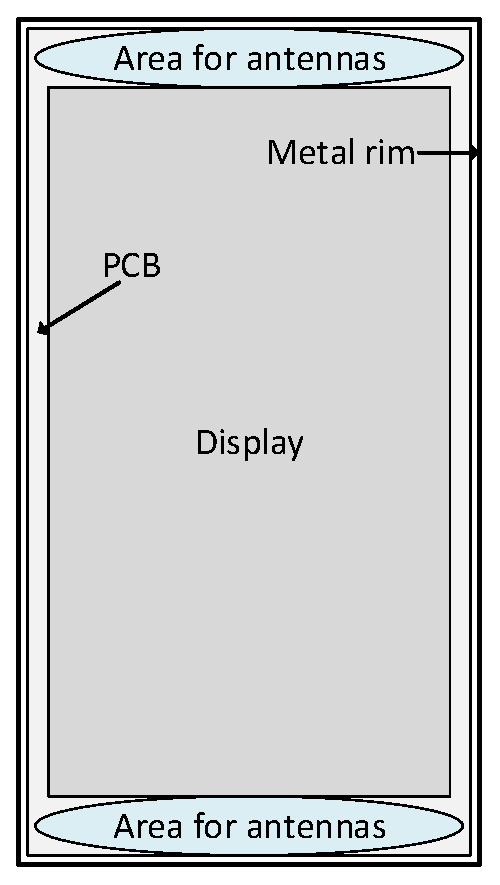
\includegraphics[width=0.9\textwidth]{img/metal_rim.eps}
        \caption{Typical locations of antennas in metal-rimmed handsets presented in \cite{ban_low_profile}.}
        \label{fig:metal_rim}
    \end{subfigure}
    \hspace{20pt}
    \begin{subfigure}[b]{0.4\textwidth}
        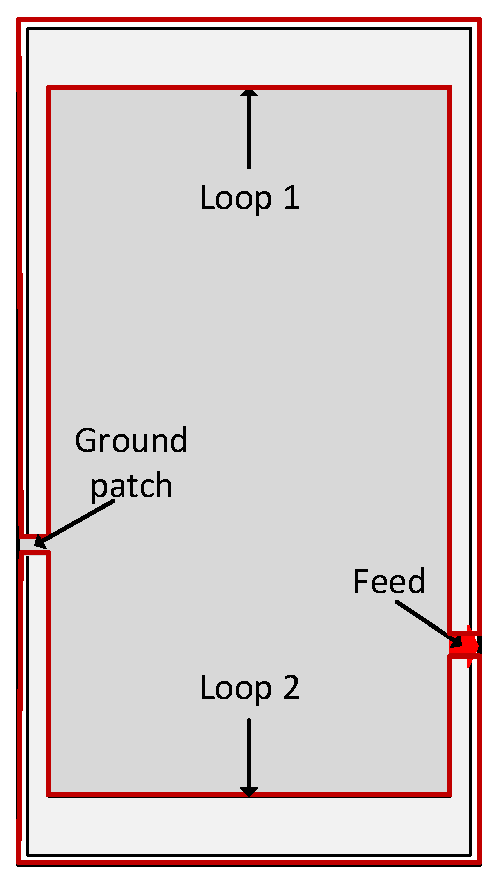
\includegraphics[width=0.9\textwidth]{img/dual_loop.eps}
        \caption{Example of a dual-loop antenna in metal-framed phone used in \cite{ban_dual_loop, stanley_lte_mimo}.}
        \label{fig:dual_loop}
    \end{subfigure}
    \caption{Proposed configurations in previous studies.}
    \label{fig:metal_rim_examples}
\end{figure}

As the display is acting as ground plane, the metal rim can be grounded with a small patch \cite{ban_dual_loop, stanley_lte_mimo}. Placing feed to another patch forms two loops between the display and the metal rim, as Figure \ref{fig:dual_loop} illustrates. This technique allows to keep the metal rim unbroken to maximize the strength of the phone. The length of the loop can be chosen such that different wave modes are excited. Since one feed-ground patch pair creates two loops of different lengths, both having own excited loop modes, this design can cover multiple frequency bands. Loops can, however, be located above the display, like traditional PIFAs \cite{reconf_narrow,hybrid}. %\cite{ban_dual_loop, stanley_lte_mimo}

Different resonant modes can be obtained also with slots in the ground plane \cite{yuan_slot}. Combining slots with loops a large number of resonance modes can be achieved \cite{hsu_compact}. Each element supports several modes that can be excited simultaneously to obtain wide bandwidth. However, slots and loops require quite large space, which is already limited. Monopole antenna in the side metal itself saves space inside the phone for other applications \cite{lee_monopole, valkonen_multifeed}. Cutting gaps to the metal rim constructs a monopole antenna, which couples with the rest of the rim to cover a wide set of frequencies \cite{chen_metal_frame}. Besides these antennas integrated into the structure, IFAs are also used \cite{hepta_ifa}. %\cite{hsu_compact, yuan_slot, lee_monopole, chen_metal_frame}

From the metal rim on the sides of the phone, the next step is metallic back cover, and full metal housing. Similarly to handsets with metal rim, metallic back cover improves robustness but deteriorates the performance of antennas. However, the harmful effects of full metal back cover are so strong, that many of the antenna solutions in the recent studies have slots in the cover (Figure \ref{fig:metal_covers}). In those studies antennas are either PIFAs, or monopoles or the slots themselves \cite{wu_pier, son_wideband_mimo, wu_tunable, zhong_pier}. 

Few studies have still shown promising antenna designs for handsets with full metal back cover. These designs are based on PIFAs or L-shaped strips, but they require a part of the metal rim to be removed \cite{chen_compact_lte, wu_pier}. These modifications make the handset not fully metal-covered, but as the metallic back cover is the main challenge in these cases, the proposed solutions are usable as they have achieved at least 40\,\% efficiency in the operating bands. %\cite{chen_compact_lte, wu_pier}

\begin{figure}[H]
\centering
    \begin{subfigure}[b]{0.3\textwidth}
        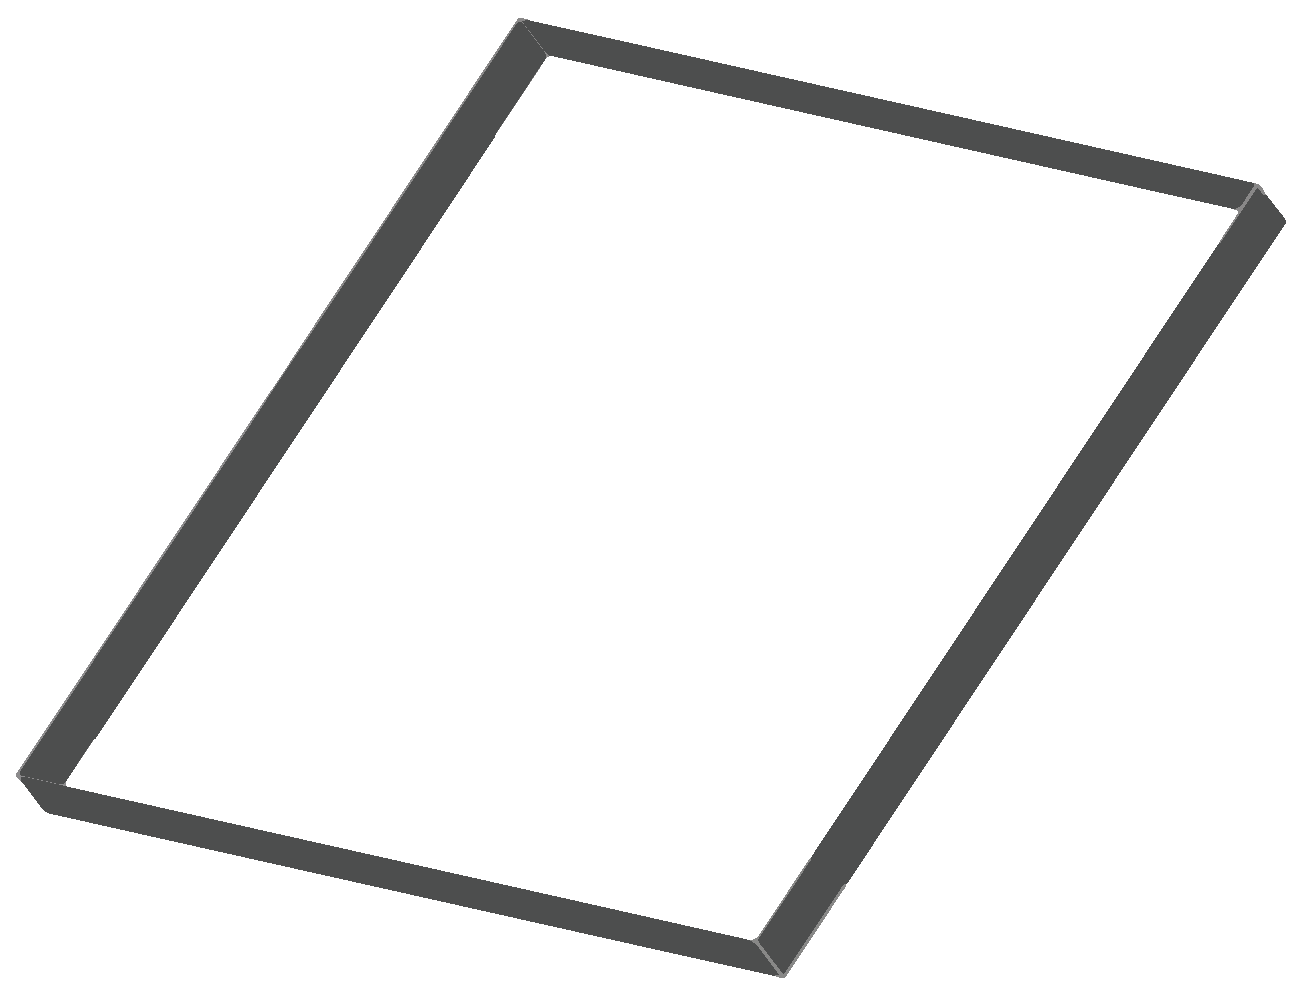
\includegraphics[width=\textwidth]{img/metal_rim2.eps}
        \caption{Metal rim.}
        \label{fig:rim}
    \end{subfigure}
    \begin{subfigure}[b]{0.3\textwidth}
        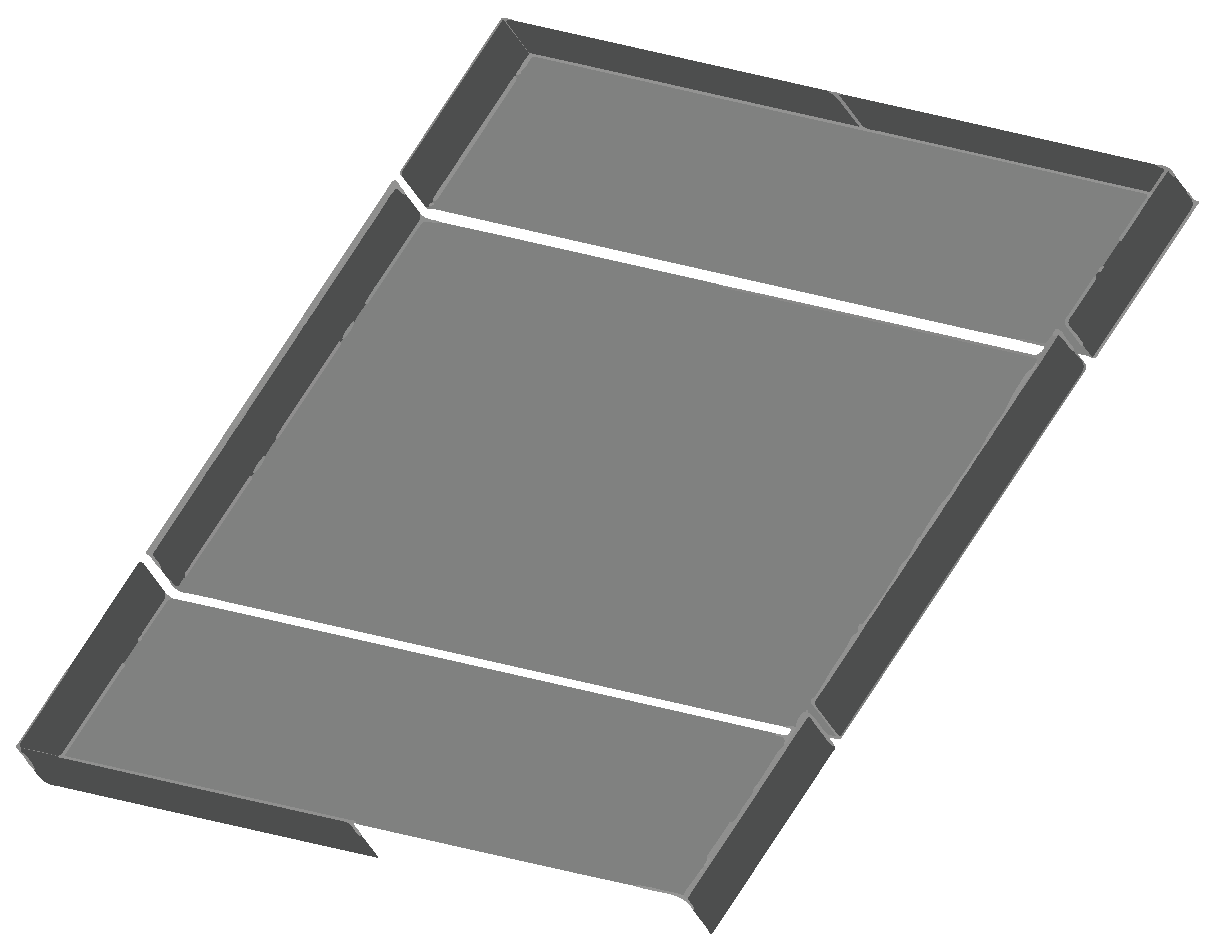
\includegraphics[width=\textwidth]{img/metal_cover_slots.eps}
        \caption{Examples of slots.}
        \label{fig:cover_slots}
    \end{subfigure}
    \begin{subfigure}[b]{0.3\textwidth}
        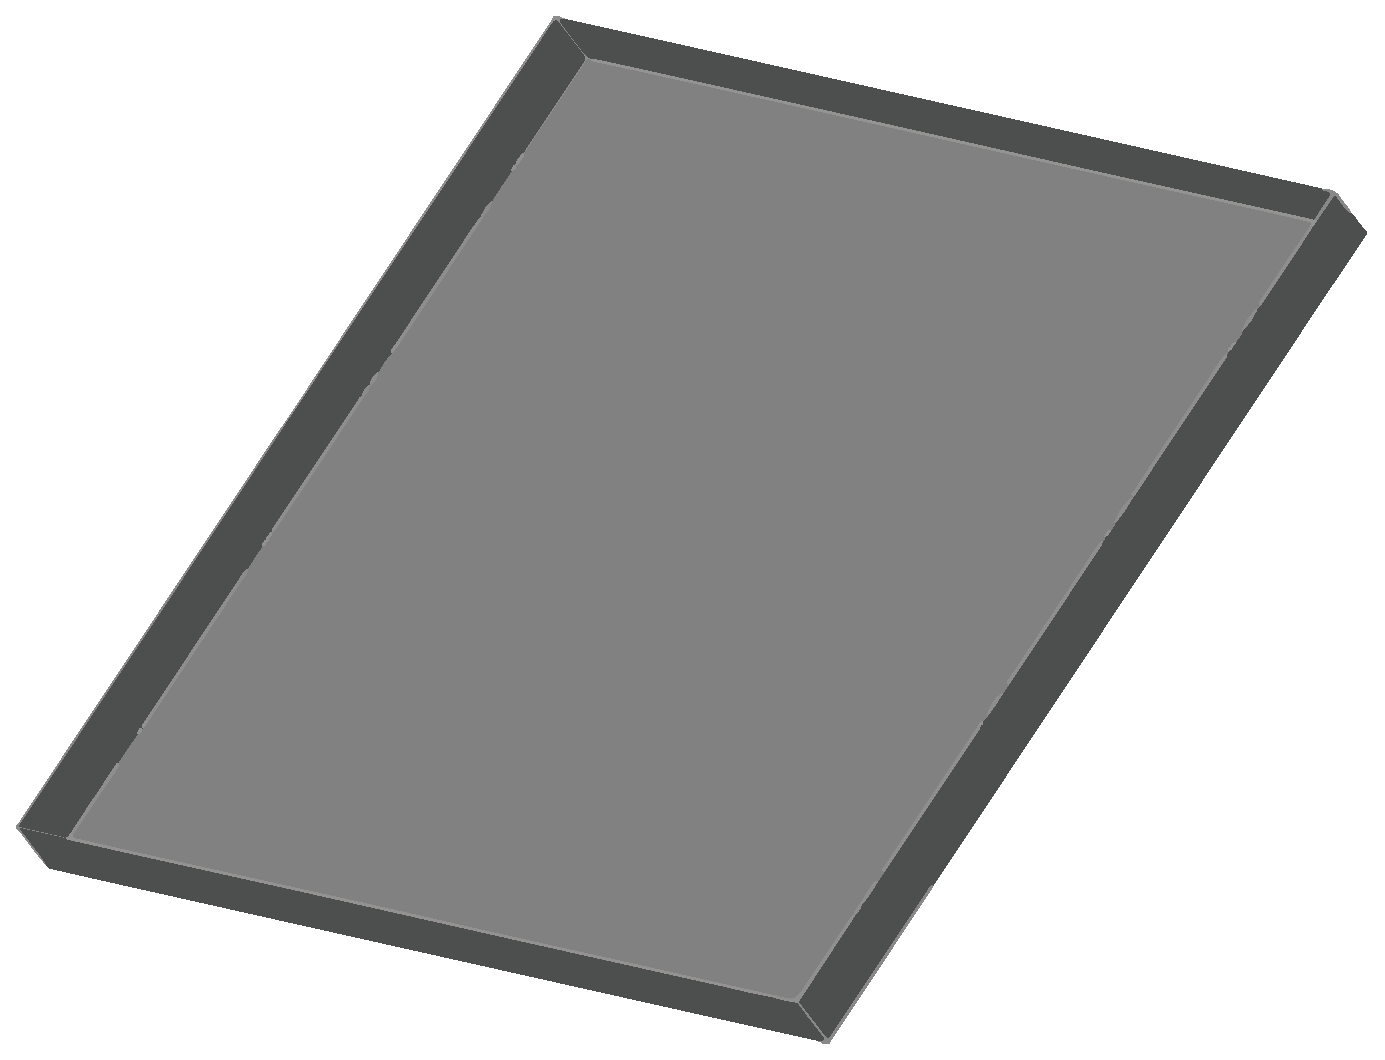
\includegraphics[width=\textwidth]{img/metal_cover_full.eps}
        \caption{Full metal cover.}
        \label{fig:full_cover}
    \end{subfigure}
    \caption{Re-illustrated examples of metal-covering of mobile phone presented in\cite{chen_compact_lte}.}
    \label{fig:metal_covers}
\end{figure}



\subsection{Key aspects in previous studies}
\label{sec:key_aspects}
More interesting matter in the previously studied antenna solutions is the technical details like operational frequencies and matching techniques, rather than positioning of antennas. \Cref{tab:metal_rim_comp,tab:metal_cover_comp} list the key details of each previously studied antenna for metal-rimmed or metal-covered phone, respectively. As can be expected of today's mobile devices, all solutions are for LTE networks. Still, only antennas proposed in \cite{stanley_lte_mimo, son_wideband_mimo, chen_compact_lte, chen_metal_frame,valkonen_multifeed} support LTE bands operating at $700-800\,\mega\hertz$. These solutions tend to have average of $40\,\%$ efficiency in the low band. 

As majority of proposed solutions operate at frequencies $800-960\,\mega\hertz$ and $1.7-2.7\,\giga\hertz$, the performance of antennas in these ranges is obviously better. Typical efficiencies on average for lower frequencies are around $50-70\,\%$ and for the high band $60-80\,\%$ \cite{ban_dual_loop,chen_compact_lte,son_wideband_mimo,chen_metal_frame,zhong_pier}. Effect of user's hand or head is also measured in \cite{zhong_pier, chen_metal_frame,ban_dual_loop,reconf_narrow,hybrid,hepta_ifa}. The effect is significant since efficiencies drop to average of $10-30\,\%$ in all supported bands. 

A common factor in nearly all of the referenced designs, is that the antennas require almost the whole width of the device. Only \cite{wu_pier,wu_tunable} have clearly smaller antennas. Usually the total volume occupied by the antenna is rather small, but the occupied area might be problematic in a design point of view. Few designs have encountered this by integrating antennas into the metallic structures, like in \cite{chen_metal_frame,lee_monopole,wu_tunable,zhong_pier}. This saves space inside the phone for other subsystems, and enables possibly larger elements to cover also the lowest frequencies. Also \cite{valkonen_multifeed} proposes an antenna structure, that could be integrated into the metal rim, but however, in the study the measurements do not include any metal covers.

Handsets with metal covers and/or frames create a challenging operational environment for antennas. Besides the physical structure of an antenna, matching circuits have a major impact on final performance. Typically matching is done with lumped elements, and common amount of them is two or three for each antenna \cite{stanley_lte_mimo, zhong_pier, wu_pier}. Matching circuits improve isolation between elements leading to better element efficiency, as well as efficiency of the whole system, since the operating frequencies of other elements can be blocked by filtering. Even though wide band matching is desirable, it might be hard to achieve with fixed matching network. As resonance tends to occur in narrow peaks, digitally tunable capacitors (DTC) are used in antennas presented in \cite{chen_compact_lte,wu_tunable} to obtain good matching level over the whole band. To improve matching even further, few designs use band-stop \cite{lee_monopole, wu_pier} or band-pass \cite{chen_metal_frame} filters, or reactive loading \cite{chen_compact_lte, chen_metal_frame} to improve antenna's bandwidth.

The common feeding mechanism in different solutions is single-feed \cite{wu_tunable, chen_metal_frame, lee_monopole, chen_compact_lte,hepta_ifa}, neverminding the number of antenna elements. Designed slot or hybrid antennas have only one feeding point, and signal couples from the fed element to the others \cite{son_wideband_mimo,hsu_compact,zhong_pier,yuan_slot}. Dual-loop antennas presented in \cite{stanley_lte_mimo,ban_dual_loop,hybrid} are excited to their wavemodes by a single feed.

Multiple feeds are used only in designs that have also other elements than slots or loops, or have the same antenna structure copied to the other end of the phone. Clearly, in those situations each element or structure is single-fed, but total number of feeds is plural \cite{stanley_lte_mimo, son_wideband_mimo,reconf_narrow}. In \cite{valkonen_multifeed}, the design has only one antenna, but that is fed from two locations. Both feeds have their own matching circuits, and one of them operates at the low band while the other at the high band. This method results terrific, wide band matching levels, and at least $55\,\%$ total efficiency.

In LTE networks, one way to increase bandwidth and throughput is applying MIMO techniques in data transmission. However, MIMO operations are not that much studied for metal-covered phones. First design, seen in \cite{son_wideband_mimo}, has two similar antenna structures in both ends of the phone consisting complex monopole and planar inverted F antennas. This structure provides full MIMO capability for all operating frequencies, although antennas' efficiencies are only ca.\ $20\,\%$ at the lowest supported frequency of $746\,\mega\hertz$. The second MIMO solution proposed in \cite{stanley_lte_mimo} has a dual-loop antenna between ground plane and side metal frame, and a capacitive coupling element (CCE) antenna. Since the CCE antenna operates only on upper frequencies ($1710-2690\,\mega\hertz$) and does not cover the lower band, the design does not have full MIMO capability. The best multiantenna perfomance is reported in \cite{reconf_narrow}. This design has a loop antenna coupled with T-shaped monopole in both ends of the phone. Additionally, both antennas have a PIN diode for reconfiguring the operating bands. The efficiencies of each antenna in each state of the diode are above $45\,\%$ for all frequencies.

Many of the proposed antenna structures are located at one end of the handset \cite{hsu_compact,yuan_slot,hybrid,lee_monopole,valkonen_multifeed,chen_metal_frame,hepta_ifa,chen_compact_lte}. All of these designs could be modified to support MIMO by copying the antenna to the other end of the phone.

\begin{sidewaystable}[H]
%\begin{table}[H]
\centering
\caption{Comparison of previously studied antennas in metal-rimmed phones. * denotes the dimension is not available.}
\label{tab:metal_rim_comp}
\begin{tabular}{|M{0.03\textheight}|M{0.11\textheight}|M{0.11\textheight}|M{0.11\textheight}|M{0.1\textheight}|M{0.06\textheight}|M{0.15\textheight}|>{\Centering\hspace*{0pt}}M{0.18\textheight}|}
    \hline
    \textbf{Ref.} & \textbf{Type} & \textbf{Volume [$\milli\meter^3$]} & \textbf{Ground plane [$\milli\meter^2$]} &\textbf{$f$ [$\mega\hertz$]} & \textbf{$\eta$ [\%]} & \textbf{Matching network} & \textbf{Notes}\\
    \hline
    \cite{ban_dual_loop} & Dual-loop & $10\times70\times0.8$, $5\times70\times0.8$ & $115\times70$ & $824-960$, $1710-2690$ & $60-80$ & N/A & Unbroken rim\\
    \hline
    \cite{hsu_compact} & U-shaped loop + T-shaped slot & $64\times8\times0.6$ & $125\times63$ & $791-960$, $1710-2690$, $3410-3800$ & $50-90$ & N/A & Unbroken rim\\
    \hline
    \cite{yuan_slot} & Slot & $56.5\times15.5\times*$ & $115\times56.5$ & $824-960$, $1710-2170$ & $60-80$ & N/A & Unbroken rim\\
    \hline
    \cite{stanley_lte_mimo} & Dual-loop + CCE & $10\times70\times0.8$, $10\times70\times0.8$, $12\times6\times0.8$ & $110\times70$ & $698-960$, $1710-2690$ & $50-90$ & $\Pi$-topology for both antennas & Unbroken rim. MIMO capable.\\
    \hline
    \cite{reconf_narrow} & Loop + monopole & $5\times70\times0.8$ & $125\times70$ & $824-960$, $1710-2690$ & $40-70$ & N/A & Unbroken rim. MIMO capable. Re\-con\-fi\-gu\-rable with PIN diode.\\
    \hline
    \cite{hybrid} & Coupled loops & $45\times5\times0.8$ & $110\times60$ & $824-960$, $1710-2690$ & $50-95$ & N/A & Rim with slot\\
    \hline
    \cite{lee_monopole} & Monopole & $50\times6.5\times0.79$ & $132\times74$ & $824-960$, $1710-2690$ & $75-85$ & F-topology + four component band-stop filter & Rim with slots. Antenna integrated to the rim.\\
    \hline
    \cite{valkonen_multifeed} & CCE & $5\times50\times5$ & $100\times50$ & $698-960$, $1710-2690$ & $55-90$ & Four components for each feed & No rim in the phone, antenna is however integrable to it. Multiple feeds.\\
    \hline
    \cite{chen_metal_frame} & Monopole & $70\times5\times5$ & $130\times70$ & $698-960$, $1710-2690$ & $50-70$ & Four elements + two component band-pass filter + one component reactive loading & Rim with slots. Antenna integrated to the rim.\\
    \hline
    \cite{hepta_ifa} & IFA & $70\times8\times0.8$ & $132\times70$ & $824-960$, $1710-2690$ & $55-80$ & N/A & Rim with slots\\
    \hline
\end{tabular}
%\end{table}
\end{sidewaystable}

\begin{sidewaystable}[H]
%\begin{table}[H]
\centering
\caption{Comparison of previously studied antennas in metal-covered phones. * denotes the dimension is not available.}
\label{tab:metal_cover_comp}
\begin{tabular}{|M{0.03\textheight}|M{0.11\textheight}|M{0.11\textheight}|M{0.11\textheight}|M{0.1\textheight}|M{0.07\textheight}|M{0.15\textheight}|M{0.18\textheight}|}
    \hline
    \textbf{Ref.} & \textbf{Type} & \textbf{Volume [$\milli\meter^3$]} & \textbf{Ground plane [$\milli\meter^2$]} & \textbf{$f$ [$\mega\hertz$]} & \textbf{$\eta$ [\%]} & \textbf{Matching network} & \textbf{Notes}\\
    \hline
    \cite{wu_pier} & Coupled monopoles & $20.5\times5\times4$ & $120\times65$ & $1560-1690$, $2410-2490$, $4950-6510$ & average $40$ or $70$ & Two component band-stop filter & Full metal housing, with opening in the corner. Only for GPS and Wi-Fi.\\
    \hline
    \cite{son_wideband_mimo} & Monopole + IFA hybrid & $64\times16\times0.8$, $64\times16\times0.8$ & N/A & $746-960$, $1710-2170$, $2300-2400$ & $20-70$ & N/A & Metal back cover with slots. MIMO capable.\\
    \hline
    \cite{wu_tunable} & ILA & $35\times8\times5.2$ & $132\times70$ & $824-960$, $1710-2170$ & $30-55$ & 2 elements + DTC & Full metal cover with slots. Antenna integrated to the housing.\\
    \hline
    \cite{zhong_pier} & Slot & $65+20\times1\times*$, $65\times1\times*$, $40\times1\times*$, $48\times1\times*$ & $110\times65$ & $824-960$, $1560-1690$, $1710-2170$, $2410-2490$ & $40-65$ & 2 elements & Full metal cover with slots. Antenna integrated to the housing.\\
    \hline
    \cite{chen_compact_lte} & Loop & $64\times8\times7$ & $116\times64$ & $700-960$, $1710-2170$ & average $45$ or $60$ & 3 elements + 2 DTCs & Full metal housing with opening at the end of the phone\\
    \hline
\end{tabular}
%\end{table}
\end{sidewaystable}

\clearpage